\chapter{Effect of Energy Storage Sizing on Intermittent Computing System Performance}
\label{Chapter:sizingeffect}

%%%%%%%%%%%%%%%%%%%%%%%%%%%%%%%%%%%%%%%%%%%%%%%%%%%%%%%%%%
%%% Section 1: Introduction 
%%%%%%%%%%%%%%%%%%%%%%%%%%%%%%%%%%%%%%%%%%%%%%%%%%%%%%%%%%

\section{Motivation} \label{section:intro}

% \IEEEPARstart{T}{o} establish a ubiquitous Internet of Things (IoT), tens of billions of devices are to be installed, and possibly at hard-to-reach locations~\cite{6064380, 7347318, 7954016, 7488250}. Using non-rechargeable batteries constrains the lifespan of these devices and brings impractical battery replacement work. Enabling IoT devices to harvest ambient energy becomes a solution to circumvent the limited battery lifespan. 

Internet of Things (IoT) devices are becoming ubiquitous, with forecasts of hundreds of billions being installed in the near future~\cite{sparks2017trillion}.
% ~\cite{7954016, sundmaeker2010vision, dave2011next} % old citations for predictions 
% ~\cite{6064380, 7347318, 7954016, 7488250}. 
They are conventionally battery-powered, thus have constrained lifespans, necessitating inconvenient periodic battery replacement. %, and many will be in hard-to-reach locations.
Energy-harvesting is a potential solution. Environmentally harvested power is, however, intrinsically variable and intermittent~\cite{4494336}. Traditionally, large energy storage devices such as rechargeable batteries or supercapacitors are used to smooth out supply variability~\cite{Kansal:2007:PME:1274858.1274870}. Unfortunately, these increase cost and device dimensions~\cite{4494753}, raise pollution concerns~\cite{LIU2014210}, and still limit lifespans~\cite{AKHTAR2015769}. 
%TODO: Look at cutting the last 3 refs in paragraph down to 1
% yet using an energy-harvesting supply without energy buffering hinders execution by frequent power interruptions. 
% Buchli:2014:DPM:2668332.2668333, Wagemann:2017:OER:3136518.3078631,
% ~\cite{5522465, Kansal:2007:PME:1274858.1274870, Jiang:2005:PEP:1147685.1147765, Simjee:2006:ELS:1165573.1165619}

%%%%%%%%%%%%%%%%%%%%%%
% Recent research has developed \textit{intermittent computing} for energy harvesting devices to maintain execution despite frequent power interruptions by saving and restoring system volatile computing state through non-volatile memory (NVM)~\cite{Ransford:2011:MSS:1950365.1950386, 10.1145/2700249, 6960060, Lucia:2015:SSP:2737924.2737978, 6341281}. 
% % In particular, if the supply voltage is charged above a restore threshold, such systems wake up and execute. 
% During active periods, the systems save volatile state (e.g. CPU registers, RAM data) into NVM either at pre-installed points (\textit{static}) or when the supply is about to fail (\textit{reactive}). If the supply voltage drops below the minimum operating threshold, the systems lose all volatile state and shut down, with data in NVM preserved. After the supply voltage recovers to a restore threshold, the systems restore the saved state from NVM and continue execution from the last saved point. Thereby, despite frequent supply interruptions, forward execution is preserved without large energy storage. 
%%%%%%%%%%%%%%%%%%%%%%

% To remove large energy storage while maintain execution despite frequent power interruptions, recent research has developed \textit{intermittent computing} (also known as \textit{intermittent computing}), which saves and restores system volatile computing state (e.g. CPU register data, RAM data) through nonvolatile memory (NVM)~\cite{Ransford:2011:MSS:1950365.1950386, 10.1145/2700249, 6960060, Lucia:2015:SSP:2737924.2737978, 6341281, 199319}. During active periods, the system volatile state is saved into NVM either at pre-installed points (\textit{static}) or just before the power supply fails (\textit{reactive})~\cite{Sliper:2019:ESR:3316781.3317812}. The volatile state is lost when the supply voltage drops below the minimum operating threshold, while the saved state in NVM is retained. The saved state is restored from NVM when the supply voltage recovers to a restore threshold, and then the execution continues from the last saved point. Therefore, forward execution is preserved without large energy storage despite frequent supply interruptions. In intermittent computing, forward progress denotes the effective program progress, as opposed to re-executed progress, lost progress, and the progress of state-saving and -restoring operations~\cite{7478428, 7056060}. The amount of forward progress directly determines application performance (e.g. program iteration rate or task completion time). 
%%%%%%%%%%%%%%%%%%%%%%%

Recently, \textit{intermittent computing systems} (ICSs) have been proposed as an alternative~\cite{doi:10.1098/rsta.2019.0158}. Instead of using large energy storage devices to sustain execution, they tolerate power interruptions by saving the state of the system into non-volatile memory (NVM) so that computation can continue when power is restored. They may save this state (e.g. CPU registers and RAM contents) either \textit{statically} at pre-defined points, or \textit{reactively} by detecting when the supply is about to fail~\cite{doi:10.1098/rsta.2019.0158}.
% ~\cite{Ransford:2011:MSS:1950365.1950386, 10.1145/2700249, 6960060, Lucia:2015:SSP:2737924.2737978, 6341281, 199319}

Static approaches save state at points determined at design or compile time, either by inserting checkpoints~\cite{Ransford:2011:MSS:1950365.1950386, 7944791} or decomposing a program into atomic tasks\footnote{Atomic operations in ICSs denote operations that should be completed in one continuous period. If an atomic operation is interrupted by a power failure, it should be re-executed rather than resumed. Examples of atomic operations include saving and restoring volatile state, transmitting and receiving packets, and sampling sequences of data from sensors.}~\cite{10.1145/3360285, Maeng:2017:AIE:3152284.3133920}. After a power interruption, progress rolls back and resumes from the last saved checkpoint or task boundary. This can introduce issues such as violation of data memory consistency, along with wasting energy on lost and re-executed progress.
% Advantages include minimizing hardware dependency, and ensuring operation atomicity.However, progress rollback and re-execution
% Static approaches save volatile state into NVM at points determined at design time or compile time, either by inserting checkpoints~\cite{Ransford:2011:MSS:1950365.1950386, 7944791, 222579} or decomposing a program into atomic tasks~\cite{10.1145/3022671.2983995, Maeng:2017:AIE:3152284.3133920}. After power interruptions, the progress rolls back and resumes from the last saved checkpoint or task boundary. Advantages of static approaches include minimizing hardware dependency and ensuring operation atomicity. However, the progress rollback and re-execution introduce violation of data memory consistency, and waste energy on lost and re-executed progress. 
% % Also, if the consumption between two successive checkpoints or task boundaries exceeds the amount that the energy storage can guarantee, the progress may never proceed due to insufficient power input. 

% \subsubsection{Reactive ICS}
Conversely, reactive approaches monitor the supply voltage and only save state when it falls below a threshold~\cite{7442814, 7849206, 7807254}, which is set high enough to reliably save state even with a total and immediate drop-off in harvested energy. They then enter a low-power mode, in many cases preserving their volatile memory and avoiding re-execution. These typically make more forward progress than static approaches, e.g. a 2.5$\times$ mean computational speedup~\cite{Maeng:2019:SPI:3314221.3314613}. 
% and memory inconsistency
% In contrast to static approaches, reactive approaches only save volatile state in NVM when supply is about to fail by monitoring supply voltage~\cite{10.1145/2700249, 6960060}. Specifically, a reactive ICS saves volatile state and enters a low-power mode (execution halted) if the supply voltage falls below a save threshold. This save threshold is set high enough to successfully save volatile state before power fails. 
% By entering the low-power mode, reactive approaches avoid re-execution and memory inconsistency, and hence typically make more forward progress than static approaches, e.g. a 2.5$\times$ mean computational speedup presented in~\cite{Maeng:2019:SPI:3314221.3314613}. 
% % In a comparison between static~\cite{Maeng:2017:AIE:3152284.3133920} and reactive~\cite{10.1145/2700249} approaches, the reactive approach demonstrates a 2.5$\times$ mean speedup on computational workloads~\cite{Maeng:2019:SPI:3314221.3314613}. Therefore, we focus on reactive ICSs for modelling and validation in this paper. 


%system computing state, e.g. CPU registers and RAM contents, into nonvolatile memory (NVM). either at pre-installed points (\textit{static methods}) or when the supply is about to fail (\textit{reactive methods})~\cite{Sliper:2019:ESR:3316781.3317812, doi:10.1098/rsta.2019.0158}. 
% The volatile state is lost when the supply voltage drops below the minimum operating threshold, while the saved state in NVM is retained. The saved state is restored from NVM when the supply voltage recovers to a restore threshold, and then the execution continues from the last saved point. 
% Therefore, forward execution is preserved. 

In ICSs, \textit{forward progress} denotes the effective application progress, excluding re-executed progress, lost progress, and state-saving and -restoring operations~\cite{7478428}. The amount of forward progress directly determines application performance, e.g. program iteration rate or task completion time. In this paper, to allow fair comparison, we define normalized forward progress as \textit{the ratio of the effective execution time to the total elapsed time}, without being restricted to a specific workload. 

%%%%%%%%%%%%%%%%%%%%%%%
% turn into the main topic now: modelling progress, improvement by sizing energy storage 
%%%%%%%%%%%%%%%%%%%%%%%

% Modelling and estimating forward progress of an energy-harvesting intermittent computing (EHIC) device is crucial to evaluation of whether the device can achieve expected performance with variable energy source conditions after deployment, while requires considerations on energy source variability and understanding of intermittent computing systems. 
% However, traditional computer models are not able to achieve this due to lack of considerations on energy source variability and understanding of intermittent computing systems. 

\begin{figure}[!t]
    \centering
    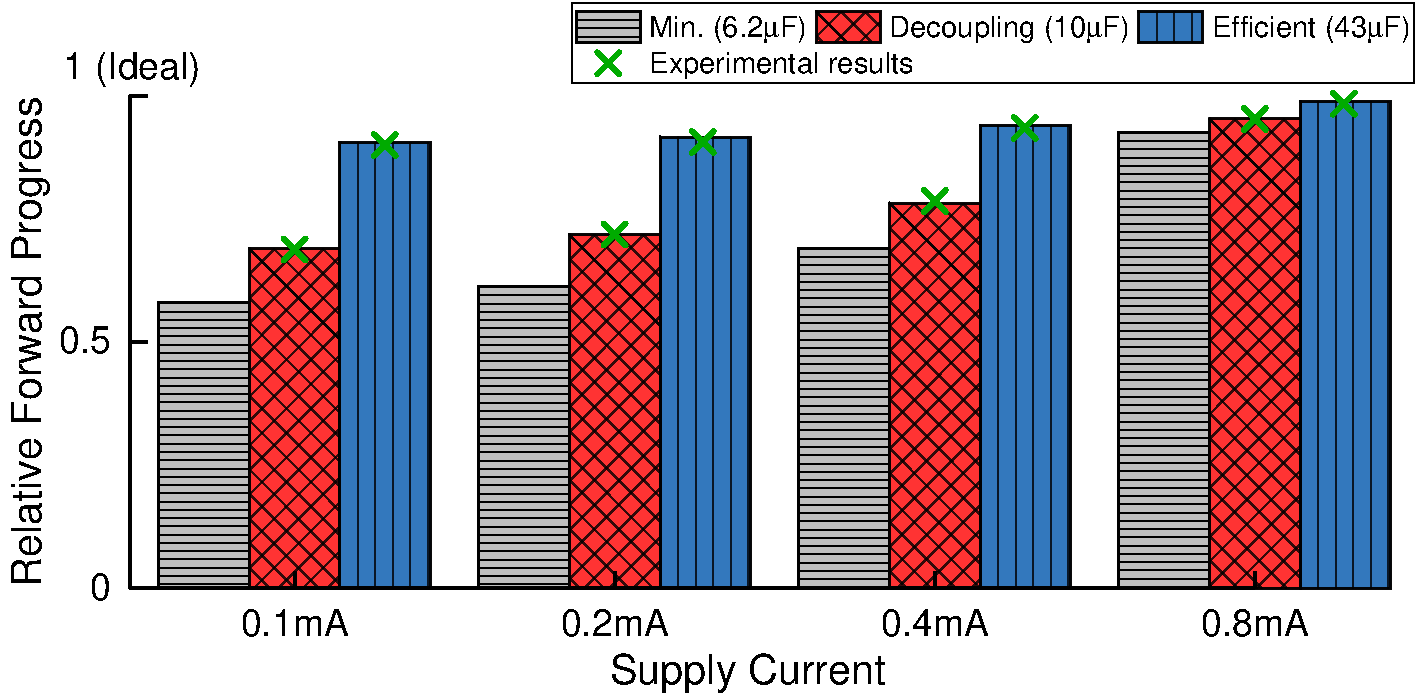
\includegraphics[width=3.33in]{ch3_sizingeffect/figures/ImprValidColorFig1}
    \caption{The relationship between energy storage capacitance and ICS forward progress, for various supply currents. }
    \label{fig:imprvalid1}
\end{figure}
% Increasing energy storage capacitance over minimum or decoupling ones can improve ICS forward progress. Results are produced by the proposed model along with experimental comparisons. 
% especially with a weak supply 

% What we did? What we did differently from them?
% We provide a modelling approach to estimate forward progress of an ICS in real-world deployment, considering energy source conditions as well as the forward progressing behaviours intermittent computing. This model can be used to explore the effect of energy harvester and energy storage sizing on forward progress. Further, we provide an approach for sizing energy storage in intermittent systems. 

With the goal of minimizing device dimensions and interruption periods, most ICS approaches adopt a minimum amount of energy storage~\cite{7442814, 10.1145/2700249, 10.1145/2809695.2809707, 10.1145/3281300, 222579}. 
This is typically just sufficient for the most energy-expensive atomic operation. 
% \cite{6960060} // hibernus
% \cite{7403941} // graceful
% \cite{10.1145/3281300} // momentum
% \cite{7442814} // hibernus++
% With the goal of minimizing device dimensions and interruption periods, previous designs in intermittent computing typically adopt only a minimum amount of energy storage, e.g. a decoupling capacitor, which is just enough for the most energy-expensive atomic operation\footnote{Atomic operations in intermittent computing denote operations that should be completed in one continuous period. If an atomic operation is interrupted by a power interruption, it should be re-executed rather than resumed. One example of atomic operations is saving and restoring volatile state. }~\cite{6960060, 7442814, 7403941, 10.1145/2700249, 10.1145/2809695.2809707, 10.1145/3281300, 222579}. 
However, our assertion is that this can be \textit{inherently inefficient in terms of time and energy}. 
We show that a system with minimum energy storage frequently goes through a cycle of: wake up, restore state, execute program, save state, and halt.
We propose that provisioning \textit{slightly more} energy storage can prolong the operating cycles, reduce the frequency of interruptions, and hence improve forward progress. We show with modelled and experimental results that (\figurename{~\ref{fig:imprvalid1}}) using efficiently-sized energy storage capacitance (\SI{43}{\micro\farad}) achieves up to a 55\% improvement in forward progress compared against using the theoretical minimum amount of capacitance (\SI{6.2}{\micro\farad}). This improvement is more significant with a weaker supply. 
%our modelled and experimental results show that 
%and \SI{30.4}{\percent}  and on-board respectively
% It achieves at least \SI{90}{\percent} of the ideal forward progress.
% However, larger energy storage also increases leakage current, occupies greater volume, and requires longer interruption periods. 
However, the relationship between ICS energy storage capacitance and forward progress has not previously been defined. Also, current tools for ICSs (Section~\ref{section:review2}) are not practical for fast estimation of forward progress in a long-term deployment, and lack a method of sizing energy storage to improve forward progress while moderating the physical size and interruption periods. 
% explored
% the challenge of sizing energy storage to improve forward progress while moderating the physical size and interruption periods is largely unaddressed.

This paper presents an approach for sizing energy storage in ICSs, quantifying and trading off forward progress, capacitor volume, and interruption periods. The main contributions are:

% when power production is less than power consumption (which is common in energy-harvesting devices). 


% We develop a theoretical model of reactive intermittent computing to estimate forward progress. Taking advantage of the theoretical model, we explore the effect of energy storage capacitance on forward progress with respect to supply current and volatile state size. We further propose an approach for identifying the proper energy storage size for deploying energy-harvesting intermittent computing (EHIC) devices, which improves forward progress while balances dimensions and interruption periods. We integrate the reactive intermittent computing model into a photovoltaic-based (PV-based) EHIC device framework. We demonstrate the sizing approach with the framework given various real-world indoor and outdoor light source datasets. 

\begin{itemize}
    \item A reactive ICS model which accurately estimates forward progress; experimental validation shows a 0.5\% mean error (Section~\ref{section:model}). %(Section~\ref{section:experiment}).
    \item A model-based sizing approach that recommends appropriate energy storage capacitance in ICSs (Section~\ref{section:approach}).
	\item An exploration based on the model, where we analyze the energy storage sizing effect on forward progress, showing up to 65\% forward progress improvement (Section~\ref{section:exploration}).     % with respect to supply current and volatile state size, 
    % while reduces capacitor volume by \SI{71.7}{\percent} and interruption periods by \SI{83.8}{\percent} as simulated with real energy availability data (Section~\ref{section:demo}). 
    % that trades off forward progress, capacitor volume, and interruption periods in ICSs . 
    \item An evaluation of the impact of sizing in real-world conditions using real energy availability data (Section~\ref{section:demo}). This includes a cost function-based method for trading off parameters. In an example, this reduced capacitor volume and interruption periods by 83\% and 91\% respectively, while sacrificing 7\% of forward progress.
    % compared to solely maximizing forward progress in simulations.%\footnote{). 
%    \color{black}
    % \item A demonstration of the sizing approach with the theoretical model integrated into a photovoltaic-based (PV-based) ICS model under various real-world light source datasets, where the suggested capacitance achieves \SI{98.3}{\percent} of the maximum forward progress while saves \SI{71.7}{\percent} capacitor volume and \SI{83.8}{\percent} interruption periods (Section~\ref{section:demo}). 
    % results show that sizing energy storage can improve annual mean forward progress by \SIrange{7.8}{43.3}{\percent}.

    % \item Experimental validation of the theoretical model, which shows high accuracy with \SI{0.5}{\percent} mean absolute percentage error, and a \SI{43}{\micro\farad} capacitor suggested by the sizing approach improves forward progress by up to \SI{55.2}{\percent} and \SI{30.4}{\percent} compared to a theoretical minimum \SI{6.2}{\micro\farad} one and an on-board \SI{10}{\micro\farad} one across various levels of supply current. 

    % \item where we found that a properly sized capacitor results in up to 30.4\% more forward progress in experiment compared to an on-board one, and improves mean forward progress by up to 35.0\% over one-year indoor and outdoor light energy harvesting simulation compared to a minimum one. 
    
    % \item experiments: which was experimentally validated with accuracy of 0.5\% mean absolute percentage error across various current input. 

    % \item We validate our formulation and model via experiments based on a TI MSP430FR6989 microcontroller, where the results show that 
\end{itemize}
%\color{blue}
% While most ICSs are designed with a minimal amount of energy storage, 
The associated simulation tool, coded in C, is available open-source at \textit{(link to be provided on publication)}. %} with real energy availability data (Section~\ref{section:demo}



% The rest of this paper is organized as follows. Background and related work on intermittent computing and its modelling approaches are provided in Section~\ref{section:review}. The device framework and the theoretical model are illustrated in Section~\ref{section:model}. The sizing approach is presented in Section~\ref{section:approach}. Model configuration and simulation setup are explained in Section~\ref{section:setup}. Design exploration and demonstration of the sizing approach are presented in Section~\ref{section:exploration}. The theoretical model is experimentally validated in Section~\ref{section:experiment}. Finally, Section~\ref{section:conclusion} concludes this paper. 

% Design considerations: forward progress, energy storage, energy harvester
% Design specifications in intermittent computing devices typically focus on three things according to applications: forward progress, interruption periods, and device dimensions. 
% interruption periods denotes the time required to wake up the device when there is power available. In some event-driven applications, interruption periods should be reduced to ensure timely event handling. Device dimensions are restricted in some size-constrained applications, for example, wearable devices or in-body sensing. Sizing energy harvester and energy storage impacts these design specifications. 

% Besides energy storage, the size of energy harvester dominates the harvested power scale. Oversized energy harvester unnecessarily increases device costs, providing excess energy beyond the necessary amount to satisfy forward progress requirement. However, there is not a method for designers to seek a cost-efficient energy harvester size to meet their design specifications in real-world deployment. 

% A general problem statement. A general summary of this work. 
% In the deployment of intermittent computing devices, it is a challenge for designers to determine the sizes of energy harvester and energy storage to both satisfy application specifications and achieve cost-efficiency. 
% perhaps explain this cost-efficiency somewhere before this place, say that using minimum storage require perhaps a large energy harvester to achieve the performance spec, but increasing storage reduce that cost without dimensional penalty. 
% In this paper, we propose a modelling approach to explore the design space in sizing energy harvester and energy storage in the deployment of intermittent computing devices. 

% \section{Related Work} \label{section:review2}

To explore forward progress of ICSs, simulation tools need to represent transient operation (timescales of \SI{}{\micro\second}-\SI{}{\milli\second}) as well as long-term overall performance (from days up to years). 

Su \textit{et al.}~\cite{Su:2019:TFR:3340300.3320270} modelled a dual-channel solar-powered nonvolatile sensor node, and Jackson \textit{et al.}~\cite{Jackson:2019:COC:3302506.3310400} provided a model to explore battery usage in ICSs. Both were configured for long-term simulations and large energy storage (from \SI{}{\milli\farad}-scale supercapacitors to batteries), thus cannot respond to frequent power interruptions and accurately estimate forward progress when using minimized energy storage (e.g. \SI{4.7}{\micro\farad}~\cite{10.1145/3281300}).

In contrast, a set of fine-grained models have been proposed to accurately simulate the frequent micro-operations in ICSs. 
NVPsim~\cite{7428003} is a gem5-based simulator for nonvolatile processors.
Fused~\cite{sliper2020fused} is a closed-loop simulator which allows interaction between power consumption, power supply, and forward progress. EH model~\cite{8574572} can compare a range of ICS approaches in a single active period with the same energy budget, quantifying forward progress by the energy spent on effective execution. These fine-grained models are inefficient for processing long-term energy data, especially when iterative tests are needed for various system configurations. 

Besides models and simulators, hardware emulators of energy harvesters~\cite{10.1145/2668332.2668336, 10.1145/3356250.3360042} can provide repeatable power profiles recorded from energy harvesters for experimental comparisons. Though they provide practical results, hardware emulations are limited by hardware options and are generally impractical for performing long-term trials.

To address the above problem, we provide a reactive ICS model to estimate forward progress, as well as a simulation tool that enables fast exploration with long-term real-world environmental conditions. Further, we provide a sizing approach which recommends appropriate energy storage capacitance for deploying ICSs. 
%%%%%%%%%%%%%%%%%%%%%%%%%%%%%%%%%%%%%%%%%%%%%%%%%%%%%%%%%%
%%% Section 3: Modelling Reactive
%%%%%%%%%%%%%%%%%%%%%%%%%%%%%%%%%%%%%%%%%%%%%%%%%%%%%%%%%%

\section{Reactive ICS Modelling} \label{sec:c3_model}

% The goal of this model is to facilitate making design decisions when deploying intermittent computing devices in real-world environments by enabling designers to observe how the sizes of energy harvester and energy storage have an impact on the key design specifications, i.e. forward progress, dimensions, and interruption periods.

% We then illustrate a formulation which describes the relationship between forward progress and energy storage capacitance given different harvested power level in reactive intermittent computing as a part of the exploration model. 

% Assumptions. low variation in harvested power, how low? what's the impact of high variance input?
To facilitate the understanding and exploration of reactive ICSs, we present a model which outputs the normalised forward progress \nm{\alpha}{exe} when powered from a constant current supply \nm{I}{harv}. Parameters of this model are listed in \tref{tab:parameter}. 
% This accounts for the \textit{Energy Storage} and \textit{Intermittent Load} modules in the system model, allowing the expected forward progress to be evaluated.
% The input parameters \nm{I}{harv} and \N{C} are related to the size configuration of energy harvester and energy storage respectively. 
% for a period of time that long enough to omit an individual uncompleted operating cycle. 
The model assumes that all configuration parameters remain constant. 

\begin{table}[!t]
    \renewcommand{\arraystretch}{1.2}
    \centering
    \caption{Model parameters of reactive ICS} 
    \label{tab:parameter}
    \begin{tabular}{|c|c|}
        % \hline
        % \textbf{Parameter} & \textbf{Description} \\
        \hline
        \multicolumn{2}{|c|}{\textbf{Input Parameters}}\\
        \hline
        \nm{I}{harv} & Energy harvester current supply\\
        \N{C}& Energy storage capacitance\\
        \hline
        \multicolumn{2}{|c|}{\textbf{Configuration Parameters}}\\
        \hline
        \nm{I}{exe} & Execution current draw\\
        \nm{I}{lpm} & Low-power mode current draw\\
        \nm{I}{r} & Restore current draw\\
        \nm{I}{s} & Save current draw\\
        \nm{I}{leak} & Leakage current draw\\
        \nm{V}{r} & Restore voltage threshold\\
        \nm{V}{s} & Save voltage threshold\\
        \nm{T}{r} & Restore time overhead\\
        \nm{T}{s} & Save time overhead\\
        \hline
        \multicolumn{2}{|c|}{\textbf{Output Parameter}}\\
        \hline
        \nm{\alpha}{exe} & Normalised forward progress \\ 
        \hline
    \end{tabular}
\end{table}

% Since supply current \nm{I}{harv} and leakage current \nm{I}{leak} constantly exist (though could be zero), 
For brevity, \nm{I}{in} denotes the usable input current as expressed in (\eref{eq:in}). The effect of capacitor leakage current, \nm{I}{leak}, is discussed at the end of \sref{subsec:formulation}.
\begin{equation}
    \nmm{I}{in} = \nmm{I}{harv} - \nmm{I}{leak}
    \label{eq:in}
\end{equation}

\subsection{Operating Modes of Reactive ICS}

The behaviour of reactive ICSs can be classified into three operating modes depending on the supply current, as shown in \fref{fig:operatingModes}. These are differentiated by the relationship between input current \nm{I}{in} and the system's current draw in its low-power mode (LPM) or active modes, i.e. \nm{I}{lpm} and \nm{I}{exe}. We define the three modes as:

\begin{figure}[!t]
    \centering
    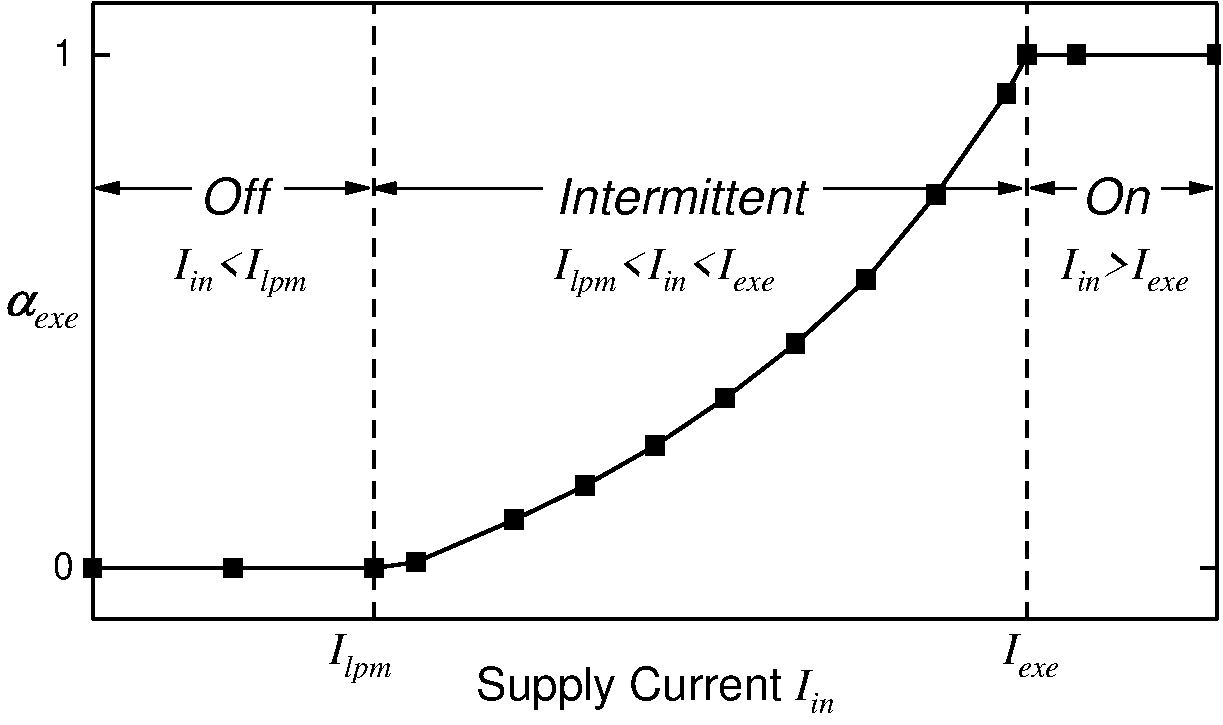
\includegraphics[width=0.8\columnwidth]{ch3_sizingeffect/figures/OperatingMode0Fig}
    \caption{Operating modes of reactive ICSs, and achieved forward progress against supply current.}
    \label{fig:operatingModes}
\end{figure}

\begin{itemize}
	\item \textit{Off} mode: When $\nmm{I}{in} < \nmm{I}{lpm}$, the system stays inactive. The supply voltage \nm{V}{cc} cannot rise above the restore threshold \nm{V}{r} to wake the system and start execution. The LPM current \nm{I}{lpm} includes the consumption of voltage monitoring circuits and system idle current.
	% Here, \nm{I}{lpm} is induced after \nm{V}{cc} goes above the minimum operating voltage $V_{off}$ where the system waits for \nm{V}{cc} to reach \nm{V}{r} (when $V_{off} < \nmm{V}{cc} < \nmm{V}{r}$). 

    \item \textit{On} mode: When $\nmm{I}{in} > \nmm{I}{exe}$, the system executes constantly as the supply voltage \nm{V}{cc} never drops below \nm{V}{s}. \nm{V}{cc} grows until \nm{I}{in} and \nm{I}{exe} are in equilibrium, which may result from \nm{I}{in} decreasing due to poor impedance matching, or \nm{I}{exe} increasing due to either greater current draw at higher voltage or dissipation through overvoltage protection circuits. 

	\item \textit{Intermittent} mode: When $\nmm{I}{lpm} < \nmm{I}{in} < \nmm{I}{exe}$, the system executes intermittently after $\nmm{V}{cc} > \nmm{V}{r}$ and before $\nmm{V}{cc} < \nmm{V}{s}$. \nm{V}{cc} can rise above \nm{V}{r} and the system starts execution. However, the stored energy is then consumed by the load as $\nmm{I}{in} < \nmm{I}{exe}$, causing \nm{V}{cc} to eventually drop below the save threshold \nm{V}{s}, where the system saves its state and enters LPM. The system stays in LPM until \nm{V}{cc} rises to \nm{V}{r} again and then resumes execution. 
	% In this mode, \nm{V}{cc} oscillates approximately between \nm{V}{r} and \nm{V}{s}, 'switching' on and off the execution. 
    In general, a higher \nm{I}{in} leads to more forward progress in this mode, but the exact relationship between \nm{I}{in} and forward progress requires further analysis.
    
	% The excess power either dissipates through circuits or overcharges \nm{V}{cc}. An overcharged \nm{V}{cc} may affect harvesting efficiency due to poor impedance matching and reduce \nm{I}{harv}, such that current input and consumption are in equilibrium. 
	% In this model case, charging \nm{V}{cc} above the maximum power point of the PV cell reduces $I_{harvest}$, and \nm{V}{cc} is stable when $I_{harvest} = \nmm{I}{exe} + \nmm{I}{leak}$. 
\end{itemize}

\subsection{Formulating Forward Progress} \label{subsec:formulation}

Next, we derive formulations to calculate \nm{\alpha}{exe} from \nm{I}{in} and energy storage capacitance \N{C}. We then explore the effect of capacitor leakage on maximum forward progress. 

In the \textit{On} and \textit{Off} modes, the normalised forward progress is trivial to find (simply 1 and 0 respectively). In the \textit{Intermittent} mode,  as shown in \fref{fig:operatingCycle}, the system goes through four intervals in turn, i.e. charging, restoring, executing, and saving, with current consumption of \nm{I}{lpm}, \nm{I}{r}, \nm{I}{exe}, and \nm{I}{s} in each interval respectively. The normalised forward progress, i.e. effective execution time ratio, is indicated as $\nmm{T}{exe} / \nmm{T}{cycle}$, where \nm{T}{exe} is the time spent on effective execution in one operating cycle and \nm{T}{cycle} is the period of operating cycles. Hence, the forward progress given all supply levels is expressed as:
\begin{equation}
    \nmm{\alpha}{exe} = \left\{
    \begin{aligned}
        & 0 & , & \quad \textit{Off} \, (\nmm{I}{in} < \nmm{I}{lpm}) \\
        & \frac{\nmm{T}{exe}}{\nmm{T}{cycle}} & , & \quad \textit{Intermittent} \, (\nmm{I}{lpm} < \nmm{I}{in} < \nmm{I}{exe}) \\
        & 1 & , & \quad \textit{On} \, (\nmm{I}{in} > \nmm{I}{exe})
    \end{aligned}
    \right.
    \label{eq:feff}
\end{equation}

\begin{figure}[!t]
    \centering
    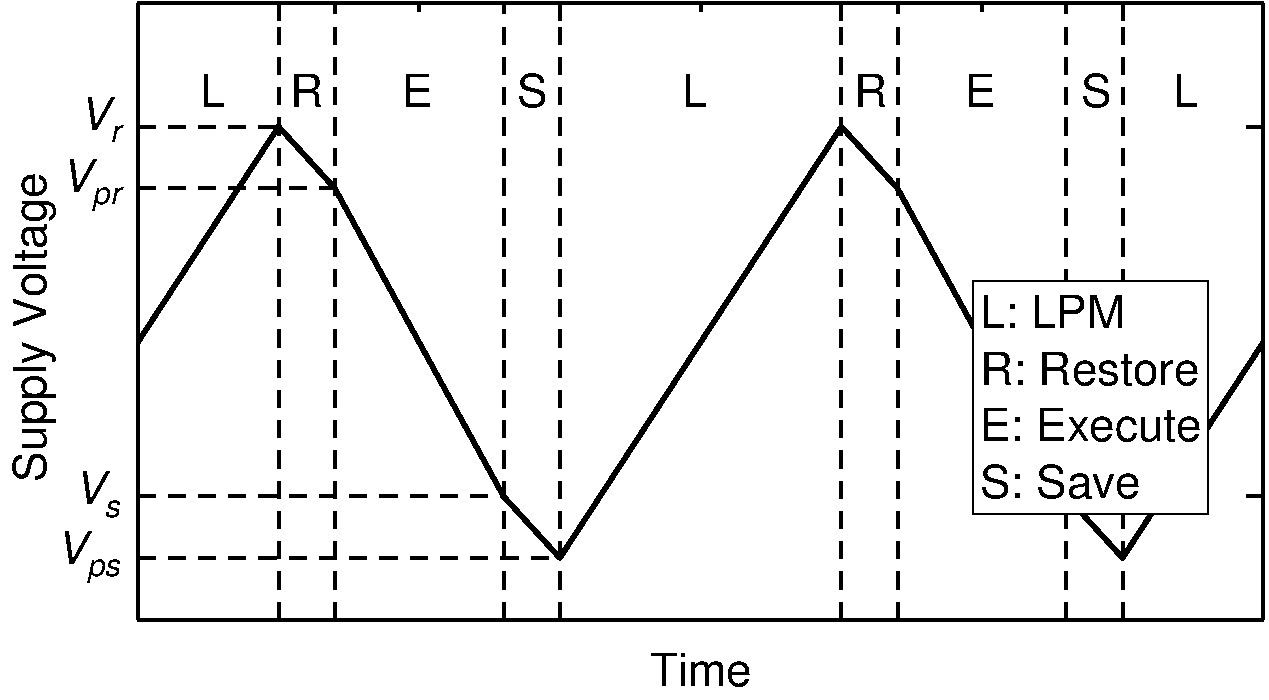
\includegraphics[width=0.8\columnwidth]{ch3_sizingeffect/figures/CRESdemoFig}
    \caption{Operating cycles in the \textit{Intermittent} mode. }
    \label{fig:operatingCycle}
\end{figure}

In the following analysis, we focus on deriving $\nmm{T}{exe} / \nmm{T}{cycle}$ in the \textit{Intermittent} mode. Let \nm{V}{pr} (post-restore) and \nm{V}{ps} (post-save) denote the voltage after restoring and saving operations. \nm{V}{pr} and \nm{V}{ps} can be calculated as:
\begin{equation}
    \nmm{V}{pr} = \nmm{V}{r} + \frac{\nmm{T}{r} (\nmm{I}{in} - \nmm{I}{r})}{C}
    \label{eq:vpr}
\end{equation}
\begin{equation}
    \nmm{V}{ps} = \nmm{V}{s} + \frac{\nmm{T}{s} (\nmm{I}{in} - \nmm{I}{s})}{C}
    \label{eq:vps}
\end{equation}
With \eref{eq:vpr}, the time spent on effective execution \nm{T}{exe} in one operating cycle can be expressed as:
\begin{equation}
    \begin{aligned}
        \nmm{T}{exe} & = \frac{C(\nmm{V}{pr} - \nmm{V}{s})}{\nmm{I}{exe} - \nmm{I}{in}} \\
        & = \frac{C(\nmm{V}{r} - \nmm{V}{s}) + \nmm{T}{r} (\nmm{I}{in} - \nmm{I}{r})} {\nmm{I}{exe} - \nmm{I}{in}}
    \end{aligned}
    \label{eq:texe}
\end{equation}
Analogously, with \eref{eq:vps}, the charging interval can be described as:
\begin{equation}
    \begin{aligned}
        T_{charge} & = \frac{C(\nmm{V}{r} - \nmm{V}{ps})}{\nmm{I}{in} - \nmm{I}{lpm}} \\
        & = \frac{C(\nmm{V}{r} - \nmm{V}{s}) - \nmm{T}{s} (\nmm{I}{in} - \nmm{I}{s})} {\nmm{I}{in} - \nmm{I}{lpm}}
    \end{aligned}
    \label{eq:tcharge}
\end{equation}
With \eref{eq:texe} and \eref{eq:tcharge}, the period of an operating cycle is:
\begin{equation}
    \begin{aligned}
        \nmm{T}{cycle} & = \quad T_{charge} + \nmm{T}{r} + \nmm{T}{exe} + \nmm{T}{s} \\
        & = \quad \frac{C (\nmm{V}{r} - \nmm{V}{s}) + \nmm{T}{s} (\nmm{I}{s} - \nmm{I}{lpm})}{\nmm{I}{in} - \nmm{I}{lpm}} + \frac{C (\nmm{V}{r} - \nmm{V}{s}) + \nmm{T}{r} (\nmm{I}{exe} - \nmm{I}{r})}{\nmm{I}{exe} - \nmm{I}{in}}
    \end{aligned}
    \label{eq:tperiod}
\end{equation}

Finally, combining \eref{eq:vpr} to \eref{eq:tperiod}, we obtain normalised forward progress \nm{\alpha}{exe} in the \textit{Intermittent} mode ($\nmm{I}{lpm} < \nmm{I}{in} < \nmm{I}{exe}$) as:
\begin{equation}
    \begin{aligned}
        \nmm{\alpha}{exe} &= \frac{\nmm{T}{exe}}{\nmm{T}{cycle}} \\
        &= [\frac{C (\nmm{V}{r} - \nmm{V}{s}) + \nmm{T}{r} (\nmm{I}{in} - \nmm{I}{r})} {\nmm{I}{exe} - \nmm{I}{in}}] / \\
        & [\frac{C (\nmm{V}{r} - \nmm{V}{s}) + \nmm{T}{s} (\nmm{I}{s} - \nmm{I}{lpm})}{\nmm{I}{in} - \nmm{I}{lpm}} + \frac{C (\nmm{V}{r} - \nmm{V}{s}) + \nmm{T}{r} (\nmm{I}{exe} - \nmm{I}{r})}{\nmm{I}{exe} - \nmm{I}{in}}] \\
    \end{aligned}
    \label{eq:texepercent}
\end{equation}
In the numerator \nm{T}{exe}, $C(\nmm{V}{r} - \nmm{V}{s})$ represents the amount of charge in the capacitor available for restoring and executing. $\nmm{T}{r} (\nmm{I}{in} - \nmm{I}{r})$ represents the charge used by a restore operation. $\nmm{I}{exe} - \nmm{I}{in}$ is the rate of charge consumption from the energy storage during execution.

% \footnote{Calculation breakdowns of differential analysis is attached in Appendix.}
% Higher \nm{\alpha}{exe} leads to more time spent on forward progress. 

% As $d\nmm{\alpha}{exe} / d\nmm{I}{in}$ is positive, higher harvested current \nm{I}{harv} leads to more forward progress. 
To explore the effect of energy storage on forward progress, we need to analyse $d\nmm{\alpha}{exe} / dC$. Here, if we assume that \nm{I}{leak} remains constant, \nm{\alpha}{exe} keeps increasing and approaches $(\nmm{I}{in} - \nmm{I}{lpm}) / (\nmm{I}{exe} - \nmm{I}{lpm})$ when energy storage capacitance \N{C} increases. Defining $(\nmm{I}{in} - \nmm{I}{lpm}) / (\nmm{I}{exe} - \nmm{I}{lpm})$ as \nm{\alpha}{exe\_ideal}, $\nmm{\alpha}{exe} = \nmm{\alpha}{exe\_ideal}$ is an ideal case, where restore and save overheads are absent.

In an electrolytic capacitor, however, \nm{I}{leak} typically increases with \N{C} with the following relationship~\cite{avxleakage}:
\begin{equation}
    \nmm{I}{leak} = kC\nmm{V}{cc}
    \label{eq:ileak}
\end{equation}
where $k$ is a constant normally in a range of \SIrange{0.01}{0.03}{\ampere\per\farad\per\volt}. Combining \eref{eq:ileak} with \eref{eq:in}, $d\nmm{I}{in} / dC$ is $-k\nmm{V}{cc}$, meaning \nm{I}{in} decreases linearly as \N{C} increases. Thus, when \N{C} increases, \nm{\alpha}{exe} keeps approaching \nm{\alpha}{exe\_ideal} while \nm{\alpha}{exe\_ideal} decreases. Hence, we believe that there is a capacitance value that leads to the maximum \nm{\alpha}{exe} considering \nm{I}{leak} increases with \N{C}.
% \cite{alcapacitor}
% Also, the time overhead of state saving and restoring operations $T_{RS\%}$ can be calculated as:
% \begin{equation}
%   T_{RS\%} = \frac{\nmm{T}{r} + \nmm{T}{s}}{\nmm{T}{exe} + \nmm{T}{r} + \nmm{T}{s}}
% \end{equation}


% In Equation~(\ref{eq:feff}), we get the relationship between forward progress and the sizes of energy harvester and energy storage. 

%%%%%%%%%%%%%%%%%%%%%%%%%%%%%%%%%%%%%%%%%%%%%%%%%%%%%%%%%%
%%% Section 5: Exploration
%%%%%%%%%%%%%%%%%%%%%%%%%%%%%%%%%%%%%%%%%%%%%%%%%%%%%%%%%%

\section{Exploration of Energy Storage Sizing} \label{section:exploration}

% This section first shows an exploration of how to improve forward progress by sizing energy storage with respect to supply current and volatile state size (Section~\ref{subsec:sizees}), and then demonstrates the sizing approach for energy storage in real-world energy source conditions. The sizing method finds the suitable energy harvester size that achieves a target forward progress and explores the energy storage sizing effect (Section~\ref{subsec:harvstor}), with a trade-off in forward progress, capacitor volume, and interruption periods (Section~\ref{subsec:tradeoff}).

In this section, we configure the reactive ICS model presented in Section~\ref{section:model} to approximate a real ICS platform, and then present an exploration of the relationship between $\alpha_{exe}$ and $C$ with respect to $I_{harv}$ and volatile state size.

\subsection{Model Configuration}

\subsubsection{Energy Storage}

The energy storage is represented as an ideal capacitor with leakage current. Its terminal voltage is directly applied to the load, so is modelled as:
\begin{equation}
  C \frac{dV_{cc}}{dt} = I_{harv} - I_{load} - I_{leak}
\end{equation}
where $I_{load}$ is the current consumption of the load. In this exploration, we refer to the empirical $I_{leak}$ of AVX TAJ low-profile series tantalum capacitors, which depends on capacitance $C$, rated voltage $V_{rated}$, and terminal voltage $V_{cc}$~\cite{avxleakage}:
% an off-the-shelf tantalum capacitor~\cite{tancap1}
\begin{equation}
    % aluminium 
%   I_{leak} = max\{0.03 C V_{rated}, \quad 4 \times 10^{-6}\}    \quad (A)
    % tantalum
    I_{leak} = 0.01 \lambda C V_{rated} \quad (A)
\end{equation}
where $\lambda$ denotes the ratio of the actual current leakage at $V_{cc}$ to the current leakage at $V_{rated}$, and $\lambda$ is approximated as: 
\begin{equation}
    \lambda = 0.05 \times 20^{\frac{V_{cc}}{V_{rated}}}
\end{equation}
We assume a typical load of $<$ \SI{4.0}{\volt} so, to minimize leakage, we select a device with $V_{rated} =$ \SI{10}{\volt} so as to operate between 25-40\% of its rated voltage~\cite{avxleakage}. 

% Here, $V_{cc}$ affects both the energy harvester and the load. On the harvester side, $V_{cc}$ is the operating voltage of PV cells, which has an effect on the harvested current $I_{harvest}$. On the load side, $V_{cc}$ is the supply voltage, which determines when the load wakes up or powers off (affecting $I_{load}$). Hence, the energy storage, the energy harvester, and the load impact on each other through $V_{cc}$, $I_{harvest}$, and $I_{load}$. 

\subsubsection{Intermittent Computing Load} \label{ssubsec:loadconfig}

The load parameters of current draws and time overheads, as listed in Table~\ref{tab:load}, were profiled with the experimental settings explained in Section~\ref{section:experiment}. 
The current draw was profiled with experimental measurements at a range of supply voltages. The variation of $I_{lpm}$ between $V_{off}$ (\SI{1.8}{\volt}) and $V_{r}$ (\SI{2.4}{\volt}) is 2\%, and for $I_{exe}$ between $V_{s}$ (\SI{2.1}{\volt}) and \SI{3.3}{\volt} is 1.5\%. $I_{exe}$ also has a run-time variation of 2.8\% due to a variable memory access rate. We omit these minor variations and use the mean of $I_{exe}$ and $I_{lpm}$ in the model. $I_{r}$ and $I_{s}$ are measured at $V_{r}$ and $V_{s}$ respectively. Given the voltage thresholds and the current consumption, the minimum energy storage capacitance is \SI{6.2}{\micro\farad}. This guarantees that a save and restore operation can complete even if the incoming supply current drops instantaneously to zero. The model parameters in Table~\ref{tab:load} are given as an example, and can be changed for different load characteristics. For example, $T_{r}$ and $T_{s}$ can be tuned for different volatile state sizes.
% $I_{exe}$ also has a run-time variation of \SIrange{-2.4}{+2.8}{\percent} 

\begin{table}[!t]
    \renewcommand{\arraystretch}{1.2}
    \centering
    \caption{Profiled MCU parameters}
    \label{tab:load}
    \begin{tabular}{|c|c|}
    \hline
    \textbf{Parameter} & \textbf{Value}\\
    \hline
    $I_{exe}$ & \SI{887}{\micro\ampere}\\
    $I_{lpm}$ & \SI{26}{\micro\ampere}\\
    $I_{r}$ & \SI{971}{\micro\ampere}\\
    $I_{s}$ & \SI{811}{\micro\ampere}\\
    $T_{r}$ & \SI{1.903}{\milli\second}\\
    $T_{s}$ & \SI{1.880}{\milli\second}\\
    % \multicolumn{2}{c}{Measured Parameters}\\
    % \hline
    % $I_{exe}, I_{R}, I_{S}$ & 0.87 mA\\
    % $I_{lpm}$ & 0.40 mA\\
    % $T_{r}$ & 2.298 ms\\
    % $T_{s}$ & 2.274 ms\\
    % \hline
    % \multicolumn{2}{c}{Simulation Parameters}\\
    % \hline
    % $I_{exe}, I_{R}, I_{S}$ & 1.00 mA\\
    % $I_{lpm}$ & 0.01 mA\\
    \hline
    \end{tabular}
\end{table}



\subsection{Sizing Energy Storage to Improve Forward Progress} \label{subsec:sizees}

% Message/Summary, How, Results. 

\subsubsection{Impact of Supply Current}

Increasing energy storage capacitance above the minimum can improve forward progress by reducing the frequency of power interruptions, but this improvement may be offset by increased leakage. \figurename{~\ref{fig:fpwconstcurr}} shows the relationship between forward progress and energy storage capacitance for a range of constant supply currents. Optimal capacitance values are shown for each current value.
% Forward progress increases with energy storage capacitance. However, , which leads to an optimal storage capacitance. 

% some more explanation about details in this graph
The minimum capacitance (dashed line in \figurename{~\ref{fig:fpwconstcurr}}) is calculated to deliver correct operation even if the supply current instantaneously drops to zero. If it does not drop to zero, this means that correct operation could have continued even with a smaller capacitance, though designing a system in this way would be inadvisable owing to unpredictability of the supply. This property is illustrated in \figurename{~\ref{fig:fpwconstcurr}}, in the area on the left of the dashed line. It may be observed that, for each of the current values, there is a sudden drop-off towards zero forward progress. This illustrates the hazard of setting the capacitance too small: the stored energy is too low to allow a restore and save to be undertaken.
%This steep fall is because the implemented control algorithm enters the low-power mode with volatile state retained after a save operation, and hence the energy used for restoring state in the first operating cycle is then used for effective execution in the following operating cycles as long as the supply voltage recovers to the restore threshold without a power interruption.
 
 % ), the execution may still progress given that the current supply keeps providing energy during execution
Typically, commercially-available capacitors have a $\pm$20\% tolerance. The effect of this variation on maximum forward progress is shown to be negligible ($<$ 0.23\%) in \figurename{~\ref{fig:fpwconstcurr}}. However, it must be pointed out that the effect would be much more pronounced if operating at the minimum capacitance as the variation of forward progress is larger with smaller capacitance values. Thus, it is recommended that a tolerance is considered when designing ICSs with minimum capacitance.

%If the volatile state is not retained in low-power mode (i.e. necessary to restore every operating cycle) or the supply only lasts for a limited period, 

% red zone: when supply current doesn't last for long. 
% (Regarding the red zone, potentially show a graph of the number of operating cycles to approximate constant current supply.)

\begin{figure}[!t]
  \centering
  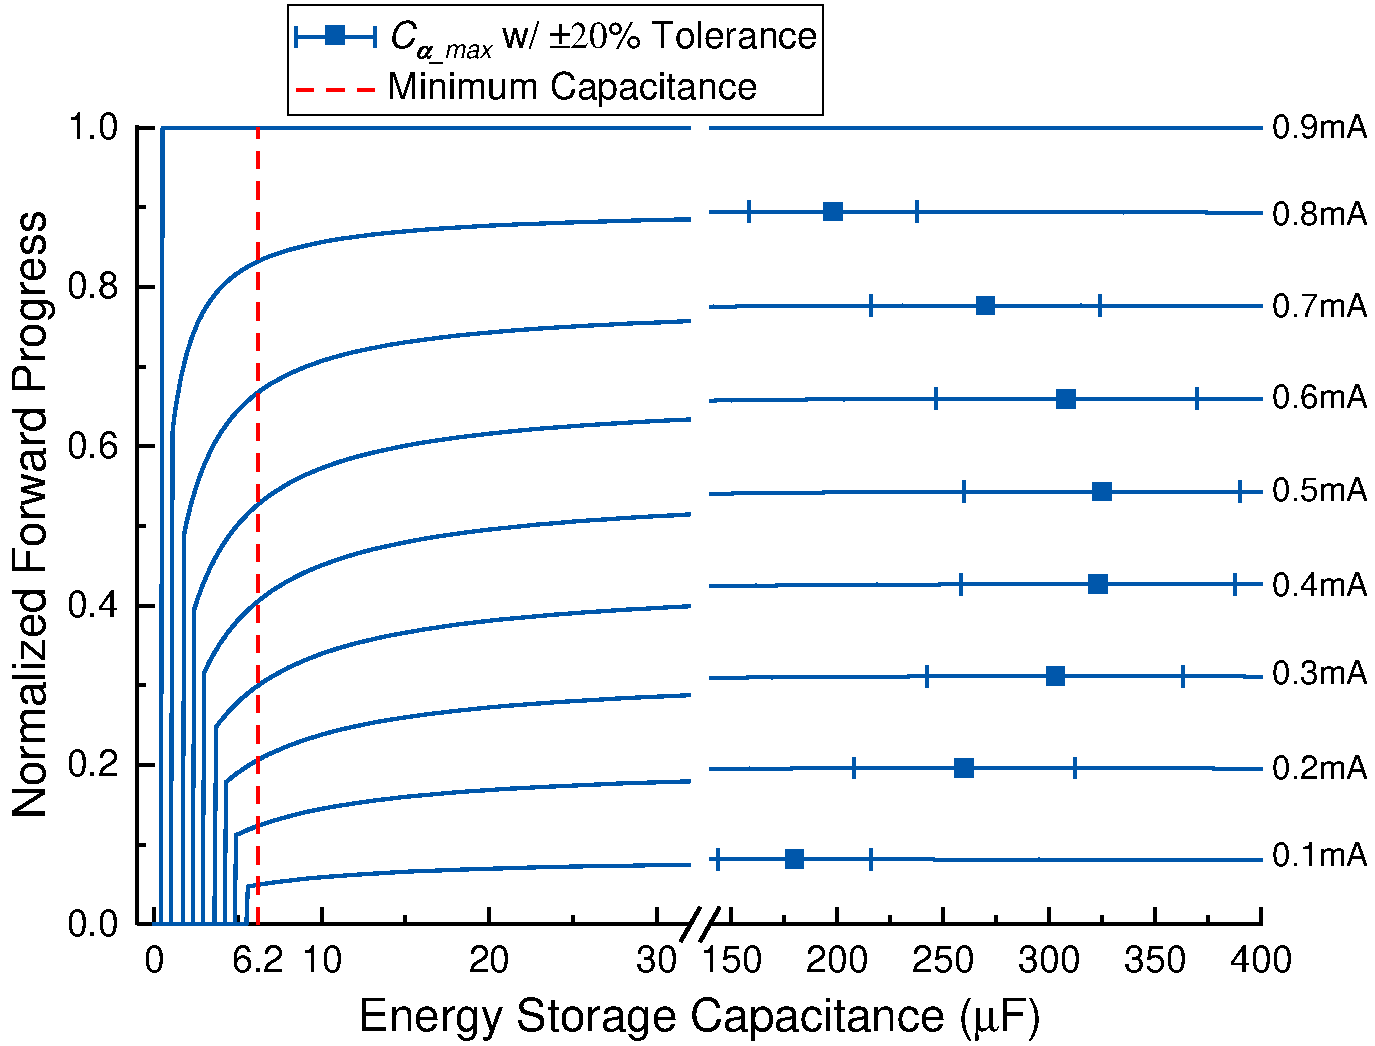
\includegraphics[width=3.2in]{ch3_sizingeffect/figures/StorCCur6Fig} 
  \caption{Forward progress against energy storage capacitance at different levels of constant supply current. Error bars around optimal points denote the impact of typical $\pm$20\% capacitance tolerance. }
  \label{fig:fpwconstcurr}
\end{figure}

\begin{figure}[!t]
  \centering
  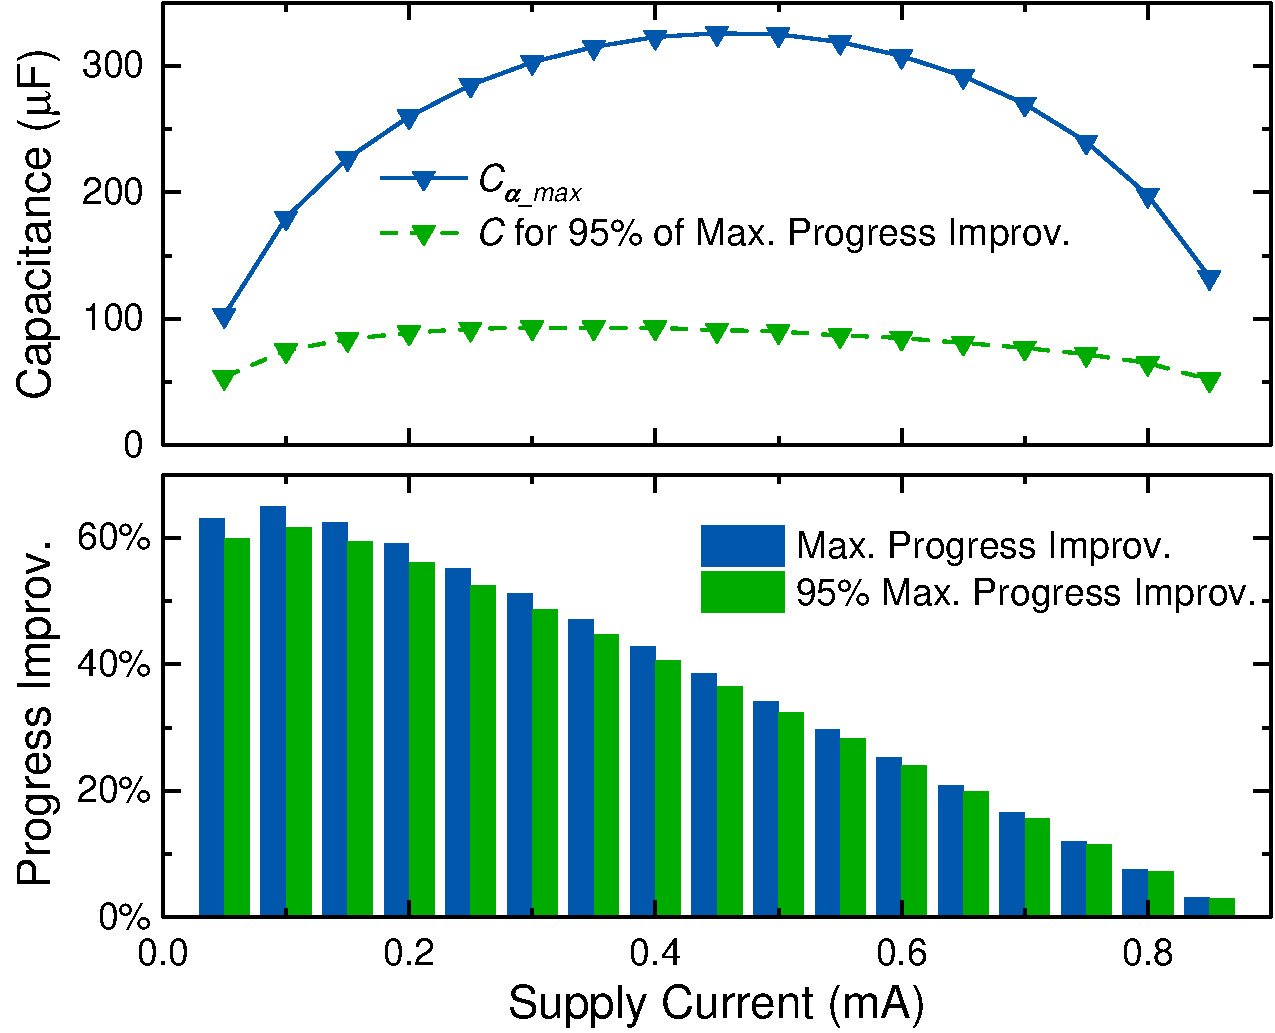
\includegraphics[width=3.2in]{ch3_sizingeffect/figures/StorCCurMax4Fig}
  \caption{Maximum forward progress improvement by sizing energy storage given a spectrum of supply current (normalized by the minimum capacitance case), with the corresponding maximum and sub-maximum (95\% of maximum) capacitance. }
  \label{fig:maxfwp}
\end{figure}

\figurename{~\ref{fig:maxfwp}} shows that an improvement in forward progress of up to 65\%  can be achieved when using the optimal capacitance instead of the minimum. However, it may not be desirable to set the capacitance solely for maximizing forward progress, because there are often trade-offs with other factors including increased interruption periods and dimensions. 
% (explored in Section~\ref{subsec:tradeoff}).
% In real-world energy source conditions, the supply current varies across this spectrum, and hence leads to an overall progress improvement based on its supply distribution. 
% This improvement exists only when the device operates in the Intermittent mode, since the device keeps either inactive in the Off mode or active in the On mode without the need for restoring and saving state. 
% Correspondingly, the optimal energy storage capacity is also plotted against supply current. 
% This optimal capacity exists because of the side effect of capacitor leakage; without capacitor leakage effect, the forward progress would keep approaching the ideal case (as explained in Section~\ref{subsec:formulation}). 
While a large improvement can be delivered with the optimal capacitance, as shown in \figurename{~\ref{fig:maxfwp}}, 95\% of this gain can still be obtained with significantly smaller capacitances (mean 31\% of the optimal value).
For example, reducing from \SI{325}{\micro\farad} to \SI{90}{\micro\farad} gives 95\% of the maximum improvement with a \SI{0.5}{\milli\ampere} supply. 

% in real deployment, storage fixed while current varies, change over a range, we may need to pick a capacity that optimise the majority of energy conditions. 

\subsubsection{Impact of Volatile State Size}

The size of volatile state differs across applications with different amounts of RAM usage, and hence incurs varying time and energy overheads for restore and save operations. We measured time overheads of restore and save operations in the minimum case (64B register data and a 160B stack) and the maximum case (64B register data and a full 2048B RAM) respectively as shown in Table~\ref{tab:ramscale}. As these time overheads are expected to be linear to the state size~\cite{Sliper:2019:ESR:3316781.3317812}, the model can be tuned for various volatile state sizes by linearly scaling the profiled values. 

% In the MCU we explore, volatile state includes CPU registers and SRAM data, which takes 64B and 160-2048B. 

\begin{table}[!t]
    \renewcommand{\arraystretch}{1.2}
    \centering
    \caption{Linear scaling range of volatile state size and restore/save time overheads}
    \label{tab:ramscale}
    \begin{tabular}{|c|cc|}
    \hline
    \textbf{State Size} & \multirow{2}{*}{\textbf{Restore Time}} & \multirow{2}{*}{\textbf{Save Time}}\\
    \textbf{(Registers + SRAM)} & & \\
    \hline
    64B + 160B (lower bound) & \SI{232}{\micro\second} & \SI{208}{\micro\second}\\
    % 64B registers + 160B stack
    64B + 2048B (upper bound) & \SI{2.298}{\milli\second} & \SI{2.274}{\milli\second} \\
    % 64B registers + 2048B RAM
    \hline
    \end{tabular}
\end{table}

An example of this is plotted in \figurename{~\ref{fig:ram}}. The forward progress improvement by sizing energy storage increases with the volatile state size, and the optimal capacitance grows accordingly. The improvement becomes insignificant when the volatile state size is small because the restore and save overheads are already negligible. For example, when the workload uses the least volatile state (the leftmost point), the maximum progress improvement is only 3.6\% although the restore and save overheads are reduced by 93\%. 
% This indicates the more efficiently ICSs save/restore, the more useless this work is. 

\begin{figure}[!t]
    \centering
    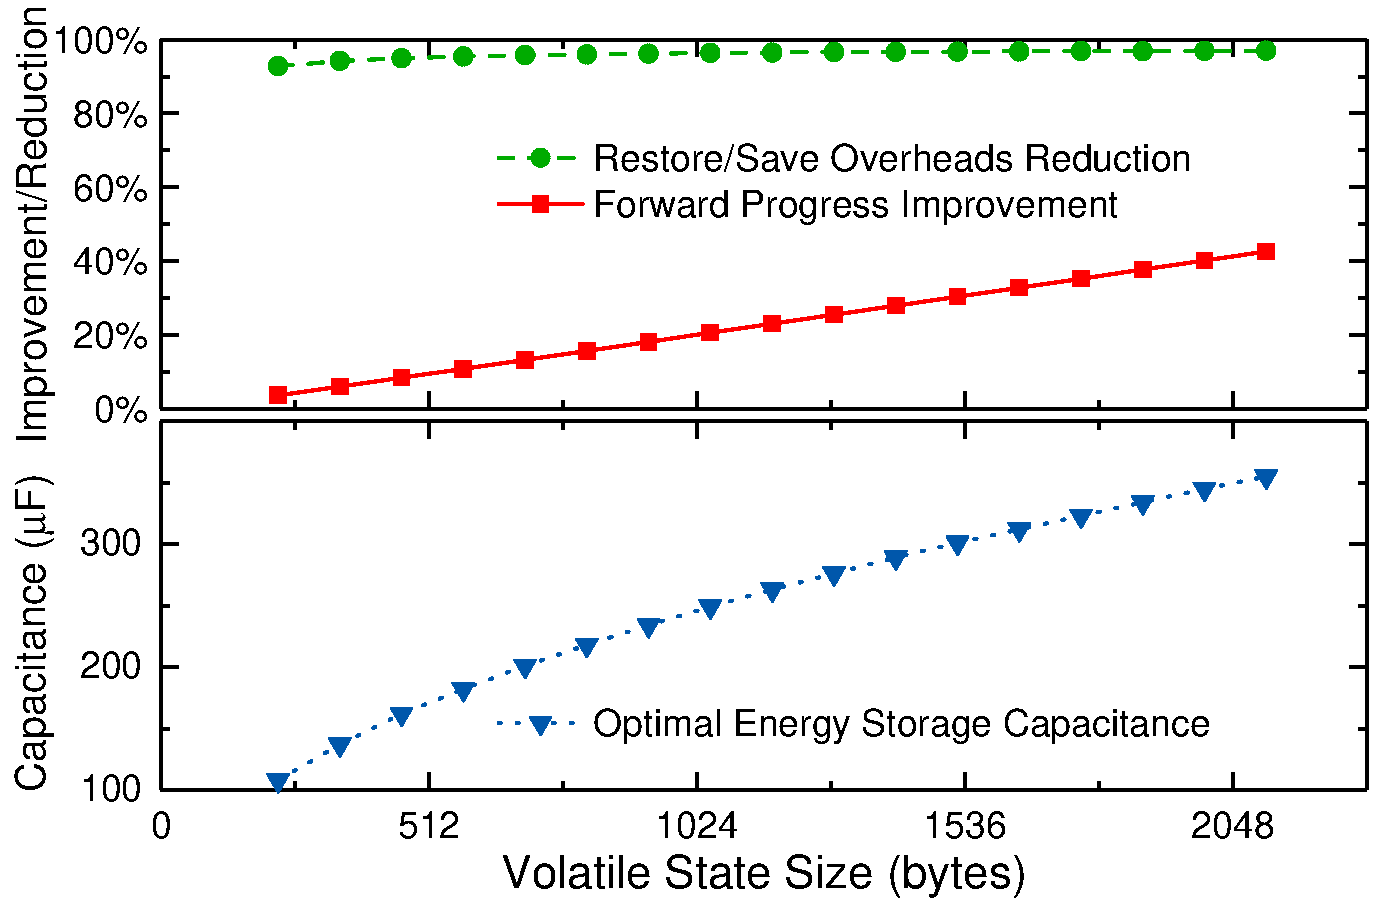
\includegraphics[width=3.2in]{ch3_sizingeffect/figures/RSTORAM3Fig}
    \caption{Impact of RAM usage (linear to restore/save overheads) on sizing energy storage with \SI{0.4}{\milli\ampere} current supply. Improvement and reduction are normalized by the minimum capacitance case. }
    \label{fig:ram}
\end{figure}

\section{Experimental Validation} \label{sec:c3_experiment}

This section compares experimental forward progress with the modelled one to validate the proposed reactive IPS model and the presented energy storage sizing effects. 

% As the sizing approach suggests the optimal energy storage capacitance in \SIrange{36}{46}{\micro\farad}, we select a \SI{43}{\micro\farad} capacitance in the experiment as an optimal value of the proposed sizing approach for comparison. 
% The forward progress with the optimal capacitance is compared to that with minimum and on-board ones, and an ideal case for a range of supply current. 
% Two goals:
% 1. To validate this model, to show that this model has high accuracy, so it can predict the forward progress reliably, across different energy storage capacitance and supply current. 
% 2. To show that the improvement / optimization of sizing energy storage given different current input conditions (so different energy source conditions). (Given our platform characteristics)

\subsection{Experiment Setup}

We validated our model on the IPS system that we parameterised for exploration (\sref{sec:c3_exploration}), so its IPS method, voltage thresholds, current draws, and workload are as mentioned.
The on-board decoupling capacitance was measured as \SI{10.0}{\micro\farad}, and hence was the minimum capacitance that could be tested. 
Further capacitance was added to provide extra energy storage up to a maximum of \SI{43}{\micro\farad}, as forward progress with this capacitance can approximate \nm{\alpha}{exe\_ideal} (an upper bound), which is linear to supply current \nm{I}{in} when $\nmm{I}{lpm} < \nmm{I}{in} < \nmm{I}{exe}$ (mentioned in \sref{subsec:formulation}).

% === The following paragraph about the actually leakage is a bit weak, so removed for now. ===
% The leakage current of these capacitors was measured to be less than \SI{10}{\nano\ampere} at \SI{3}{\volt}, which is negligible compared to the \SI{}{\micro\ampere}-level current consumption of the platform; hence we omit capacitor leakage in the following experiment and model output. However, this is only applicable to the capacitors and the capacitance range in this experiment; we consider that a leakage model is still necessary for general application.
% the specific leakage current we measured does not deny that \SI{}{\micro\ampere}-level leakage may exist in most electrolytic capacitors;

In the experiment, the task completion rate, i.e. the number of tasks completed per second, is used as the metric of forward progress rather than the effective execution time ratio. 
To gain the task completion rate from the model, we multiply the normalised forward progress (execution time ratio) generated from our model by the completion rate when the system executes constantly. 

\subsection{Model Validation} 

\begin{figure}
	\centering
	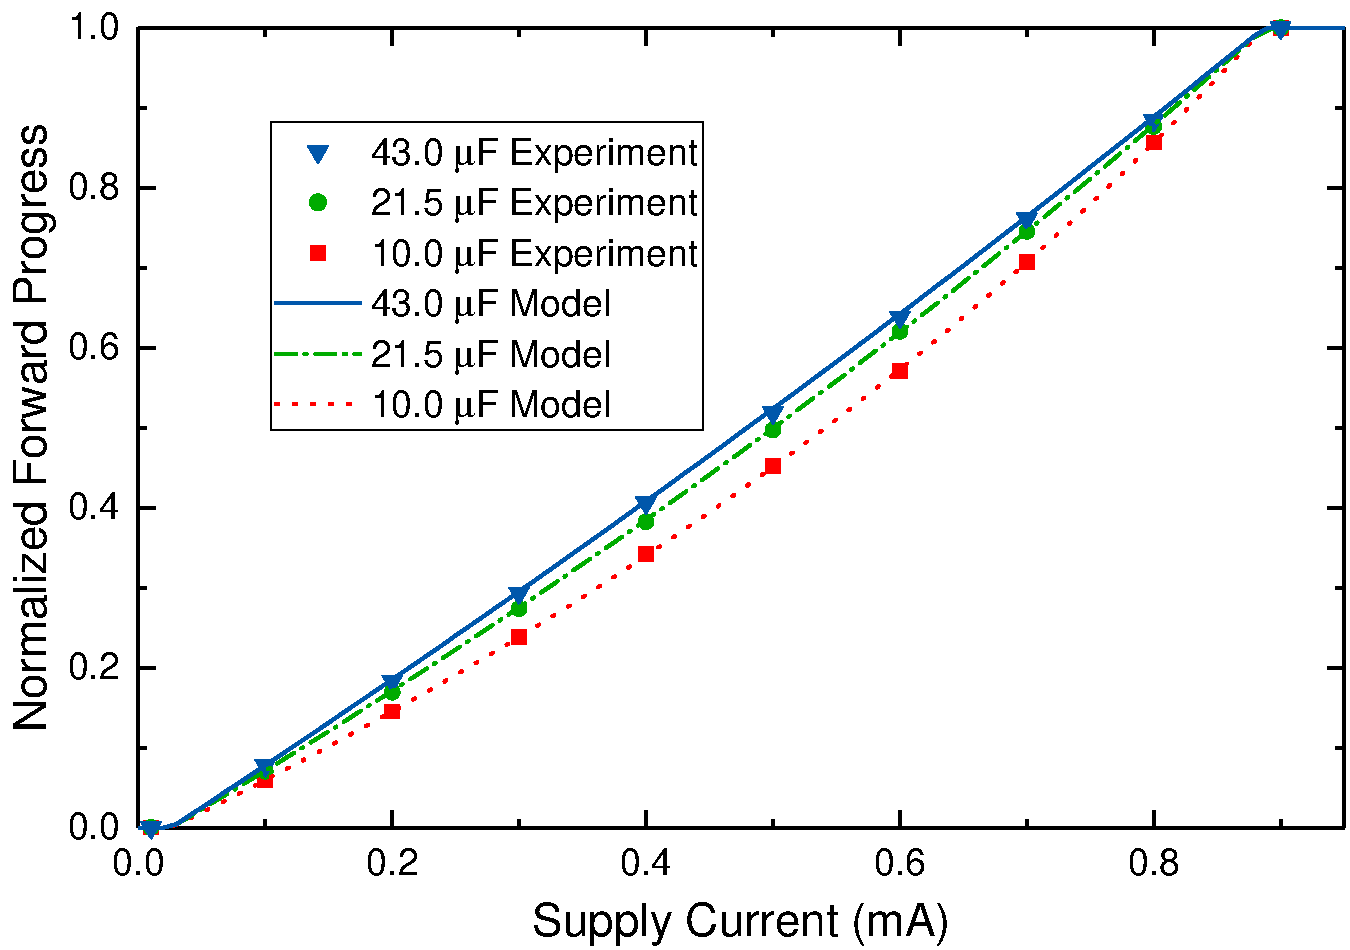
\includegraphics[width=\columnwidth]{ch3_sizingeffect/figures/ModelValidFig}
	\caption{Model validation with experimental and modelled forward progress. }
	\label{fig:modelvalid}
\end{figure}

To validate the accuracy of our model, we powered the device with a range of supply currents (\SIrange{0}{0.9}{\milli\ampere}) to operate the device in \textit{Intermittent} mode, and repeated the tests with three energy storage capacities: a) \SI{10.0}{\micro\farad} decoupling capacitance; b) \SI{21.5}{\micro\farad} (\SI{11.5}{\micro\farad} added); c) \SI{43.0}{\micro\farad} (\SI{33.0}{\micro\farad} added).
We compared the actual forward progress against predictions generated from our model. 
As shown in \figurename{~\ref{fig:modelvalid}}, the model-generated forward progress matches closely with the experimental results with only 0.5\% mean absolute percentage error across all the results. 
Hence, the proposed model is able to accurately estimate forward progress for design exploration. 

\subsection{Validation of Sizing Effects}

\begin{figure}
    \centering
    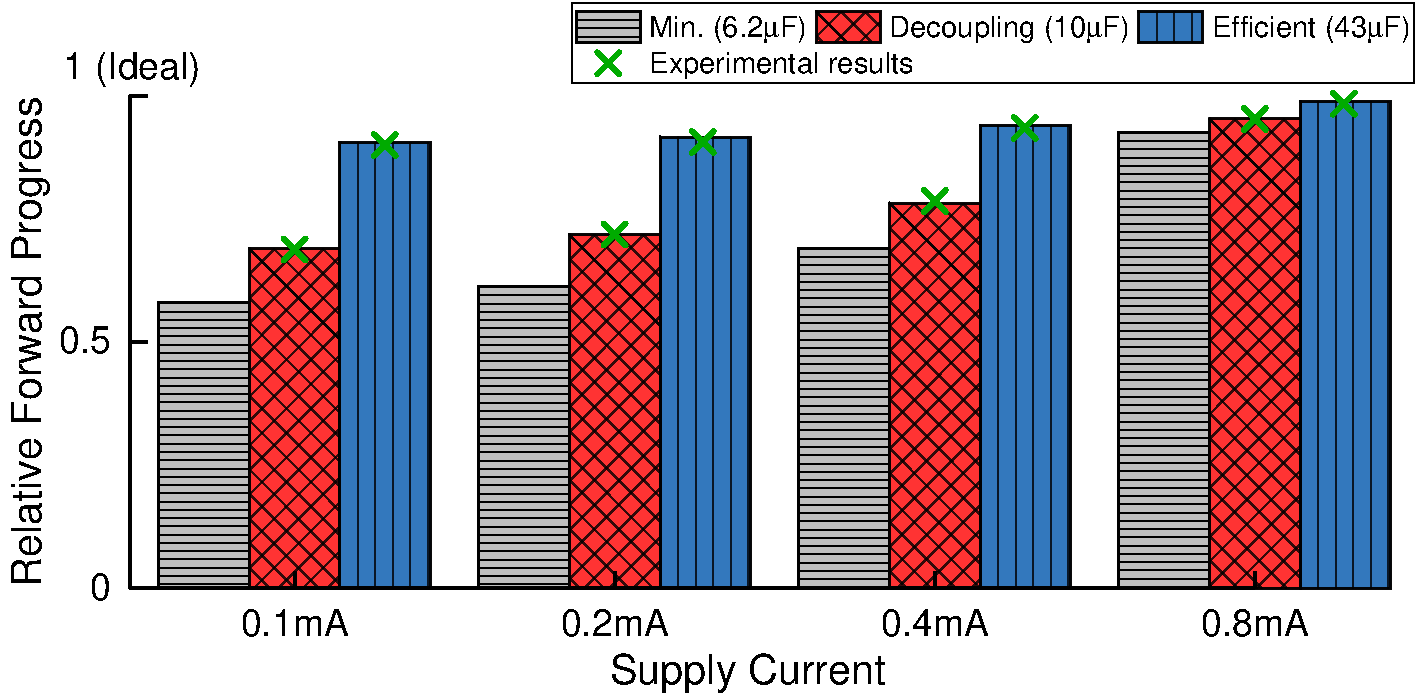
\includegraphics[width=\columnwidth]{ch3_sizingeffect/figures/ImprValidColorFig1}
    \caption{The relationship between energy storage capacitance and IPS forward progress, for various supply currents. }
    \label{fig:imprvalid1}
\end{figure}

As shown with modelled and experimental results in \fref{fig:imprvalid1}, the efficiently-sized energy storage capacitance (\SI{43}{\micro\farad}) improves forward progress by up to 55\% and 30\% compared against using the minimum and decoupling capacitance respectively. 
We notice that this improvement becomes significant when the supply current attenuates because the save and restore overheads consume a larger proportion of the available energy. 
Also, the efficiently-sized capacitor achieves at least 90\% of the ideal forward progress across the tested supply currents.
The ideal case only switches between LPM and execution, without restoring and saving overheads (explained in \sref{subsec:formulation}). 
These results illustrate the importance of this technique, in particular for conditions where the supply current is low.


\section{Summary}

While conventional ICSs have used minimal levels of capacitance, this paper has shown that increasing the amount of energy storage can improve forward progress by up to 65\% with a constant current supply and 43\% with real-world PV sources. The work includes a simulation tool which is available to download, enabling researchers to experiment with energy storage sizes to optimize ICS designs. A cost function can be incorporated, allowing various properties of the system to be traded-off. Our conclusion is that energy storage should be carefully designed, rather than minimized or indiscriminately picked, to efficiently operate ICSs. Future work will include a further investigation into cost functions for meeting multiple design objectives, and extensions to the simulation tool, e.g. models of additional energy storage devices and peripheral workloads.